%\documentclass[preprint,3p,times,twocolumn]{elsarticleUS}
\documentclass[review,3p,times]{elsarticleUS}
\usepackage{amssymb}
\usepackage{amsmath}
\usepackage{graphicx}
\usepackage{bm}
\usepackage{yhmath}
\usepackage{subfigure}
\usepackage{multirow}
\usepackage{color}
\usepackage{xcolor}
\usepackage{subdepth}
%\usepackage[nomarkers,lists]{endfloat}

\def\pp#1#2{\frac{\partial #1}{\partial #2}}

\biboptions{comma,sort&compress}

\journal{Combustion and Flame}

\makeatletter
\def\@author#1{\g@addto@macro\elsauthors{\normalsize%
    \def\baselinestretch{1}%
    \upshape\authorsep#1\unskip\textsuperscript{%
      \ifx\@fnmark\@empty\else\unskip\sep\@fnmark\let\sep=,\fi
      \ifx\@corref\@empty\else\unskip\sep\@corref\let\sep=,\fi
      }%
    \def\authorsep{\unskip,\space}%
    \global\let\@fnmark\@empty
    \global\let\@corref\@empty  %% Added
    \global\let\sep\@empty}%
    \@eadauthor={#1}
}
\makeatother

\begin{document}

\begin{frontmatter}

\title{NTC-Affected Ignition of DME by Heated Counterflowing Air}

\author{Sili~Deng}
\author{Peng~Zhao}
\author{Delin~Zhu}
\author{Chung K.~Law\corref{cor}}
\cortext[cor]{Corresponding Author: cklaw@princeton.edu}

\address{Department of Mechanical and Aerospace Engineering, Princeton University, Princeton, NJ 08544, USA}


\begin{abstract}
An experimental study, supported by computation, was conducted on the coupling of NTC-chemistry and transport in low-temperature ignition, using the nonpremixed counterflow which provided a well-characterized flow time for comparison with the chemical ignition delay time.  In particular we were interested to explore if ignition in a strained flow field with a finite residence time could still be fundamentally affected by the low-temperature NTC chemistry, as recently computationally demonstrated for the nonpremixed counterflow of heptane versus heated air. The fuel chosen in this study is dimethyl ether (DME). The presence of low-temperature reactivity was detected by using a photomultiplier tube (PMT) which measured the chemiluminescense from the radicals generated by the low-temperature chemistry. A filter combined with the PMT captured the spectrum around 400 nm, corresponding to the radiation emission of the HCHO molecules. The signal is further processed by a lock-in amplifier to diminish the noise. A highly sensitive infrared camera was also used to visualize the mixing reaction layer, with images clearly showing the diffusion cool flame. Experiments conducted under various fuel boundary concentrations and strain rates showed that ignition affected by the NTC chemistry, relevant at lower air boundary temperatures, was achieved at lower strain rates, and was found to be insensitive to a wide range of fuel concentrations. Both experimental findings agreed well with the computation using detailed chemistry, with the controlling mechanisms identified.
\end{abstract}

\begin{keyword} 
Negative Temperature Coefficient (NTC) \sep DME \sep
Nonpremixed counterflow
\end{keyword}

\end{frontmatter}

%\clearpage % For word count
\section{Introduction}

Negative temperature coefficient (NTC) refers to the phenomenon that the ignition delay time of a fuel/air mixture increases with increasing initial temperature within a certain low-temperature range. For example, at $1$ atm this range is between $600$ and $800$ K. It indicates that the reactivity of the mixture is non-monotonic to temperature variation, being stronger at lower temperatures. Since it is so essential to the combustion of most hydrocarbon fuels, especially for processes associated with engine knock, the NTC phenomenon has been extensively studied. Most of these studies, however, employed homogenous systems, such as shock tube~\cite{ciezki93}, flow reactor~\cite{wada11}, jet stirred reactor~\cite{veloo13}, and rapid compression machines~\cite{mittal08}.

Since non-uniformities invariantly exist in realistic combustion systems, the coupling between the NTC chemistry and convective-diffusive transport processes should be considered. It is reasonable to expect that when the transport time scale becomes comparable to that of the NTC chemical time scale, the two processes will be strongly coupled. By the same reasoning, when the residence time becomes long enough, the NTC chemistry will be decoupled from transport processes and the system response will recover that of the homogenous system. Indeed, Law and Zhao~\cite{law12} have recently identified the NTC-affected ignition phenomenon in the counterflow system based on simulation and computational diagnostics, showing the existence of a secondary S-curve, with distinctive ignition and extinction turning points controlled by NTC-chemistry, grafted onto the lower branch of the primary S-curve. Furthermore this secondary S-curve becomes more pronounced at lower strain rates and higher pressures.

The primary objective of the present investigation is to experimentally explore if the subject phenomenon, computationally predicted, indeed exists, and to characterize its response if the exploration is affirmative. The investigation is a challenging one because of the weak reactivity and exothermicity involved, rendering unambiguous detection difficult.

Dimethyl ether (DME) was selected as the fuel for the present study because it is gaseous and is one of the simplest hydrocarbons exhibiting the NTC behavior. Furthermore, detailed reaction mechanisms for low and high temperature DME oxidation~\cite{curran98,fischer00,curran00,zhao08} have been developed and validated against burner stabilized flames~\cite{kaiser00}, nonpremixed counterflow flame ignition~\cite{zheng05}, laminar flame speeds~\cite{qin05}, and rapid compression machines~\cite{mittal08}, allowing computational simulation and thereby guidance and verification of the experimentation. In particular, the present computation was conducted using a skeletal mechanism of $39$ species~\cite{bansal11} reduced from the well-validated detailed mechanism of Zhao \emph{et al.}~\cite{zhao08}. On the practical side, it is noted that due to its low-sooting characteristics and the capacity to be mass produced from natural gas and biomass, DME has been proposed as a promising alternative diesel fuel and fuel additive for reducing particulate emissions.

\section{Experimental Investigation}

A schematic of the experimental system is shown in Fig.~\ref{fig:setup}. Detailed descriptions of the counterflow experimental apparatus are given in~\cite{fotache95,liu10a}. Briefly, the counterflow apparatus consists of two vertically oriented opposing quartz nozzles with diameters of $20$ mm and separated by $20$ mm. A heated air or N$_2$ stream is issued from the upper nozzle and impinges against a room-temperature N$_2$-diluted DME steam issued from the lower nozzle. Both upper and lower streams are shielded by coflowing N$_2$ to diminish disturbance from the environment. An uncoated K-type (Chromel-Alumel) thermocouple is used to measure the maximum temperature at the upper nozzle exit. In a typical counterflow ignition experiment, ignition is achieved by gradually increasing the air boundary temperature until a flame appears. The exit temperature, measured by a thermocouple with radiation correction~\cite{zheng06}, is then defined as the ignition temperature. Single-point laser Doppler velocimetry (LDV) is used to measure the axial flow velocity along the centerline to determine the local strain rate of the flow.

\begin{figure}[ht]
  \centering
  \scriptsize
  \vspace{-0.1in}
  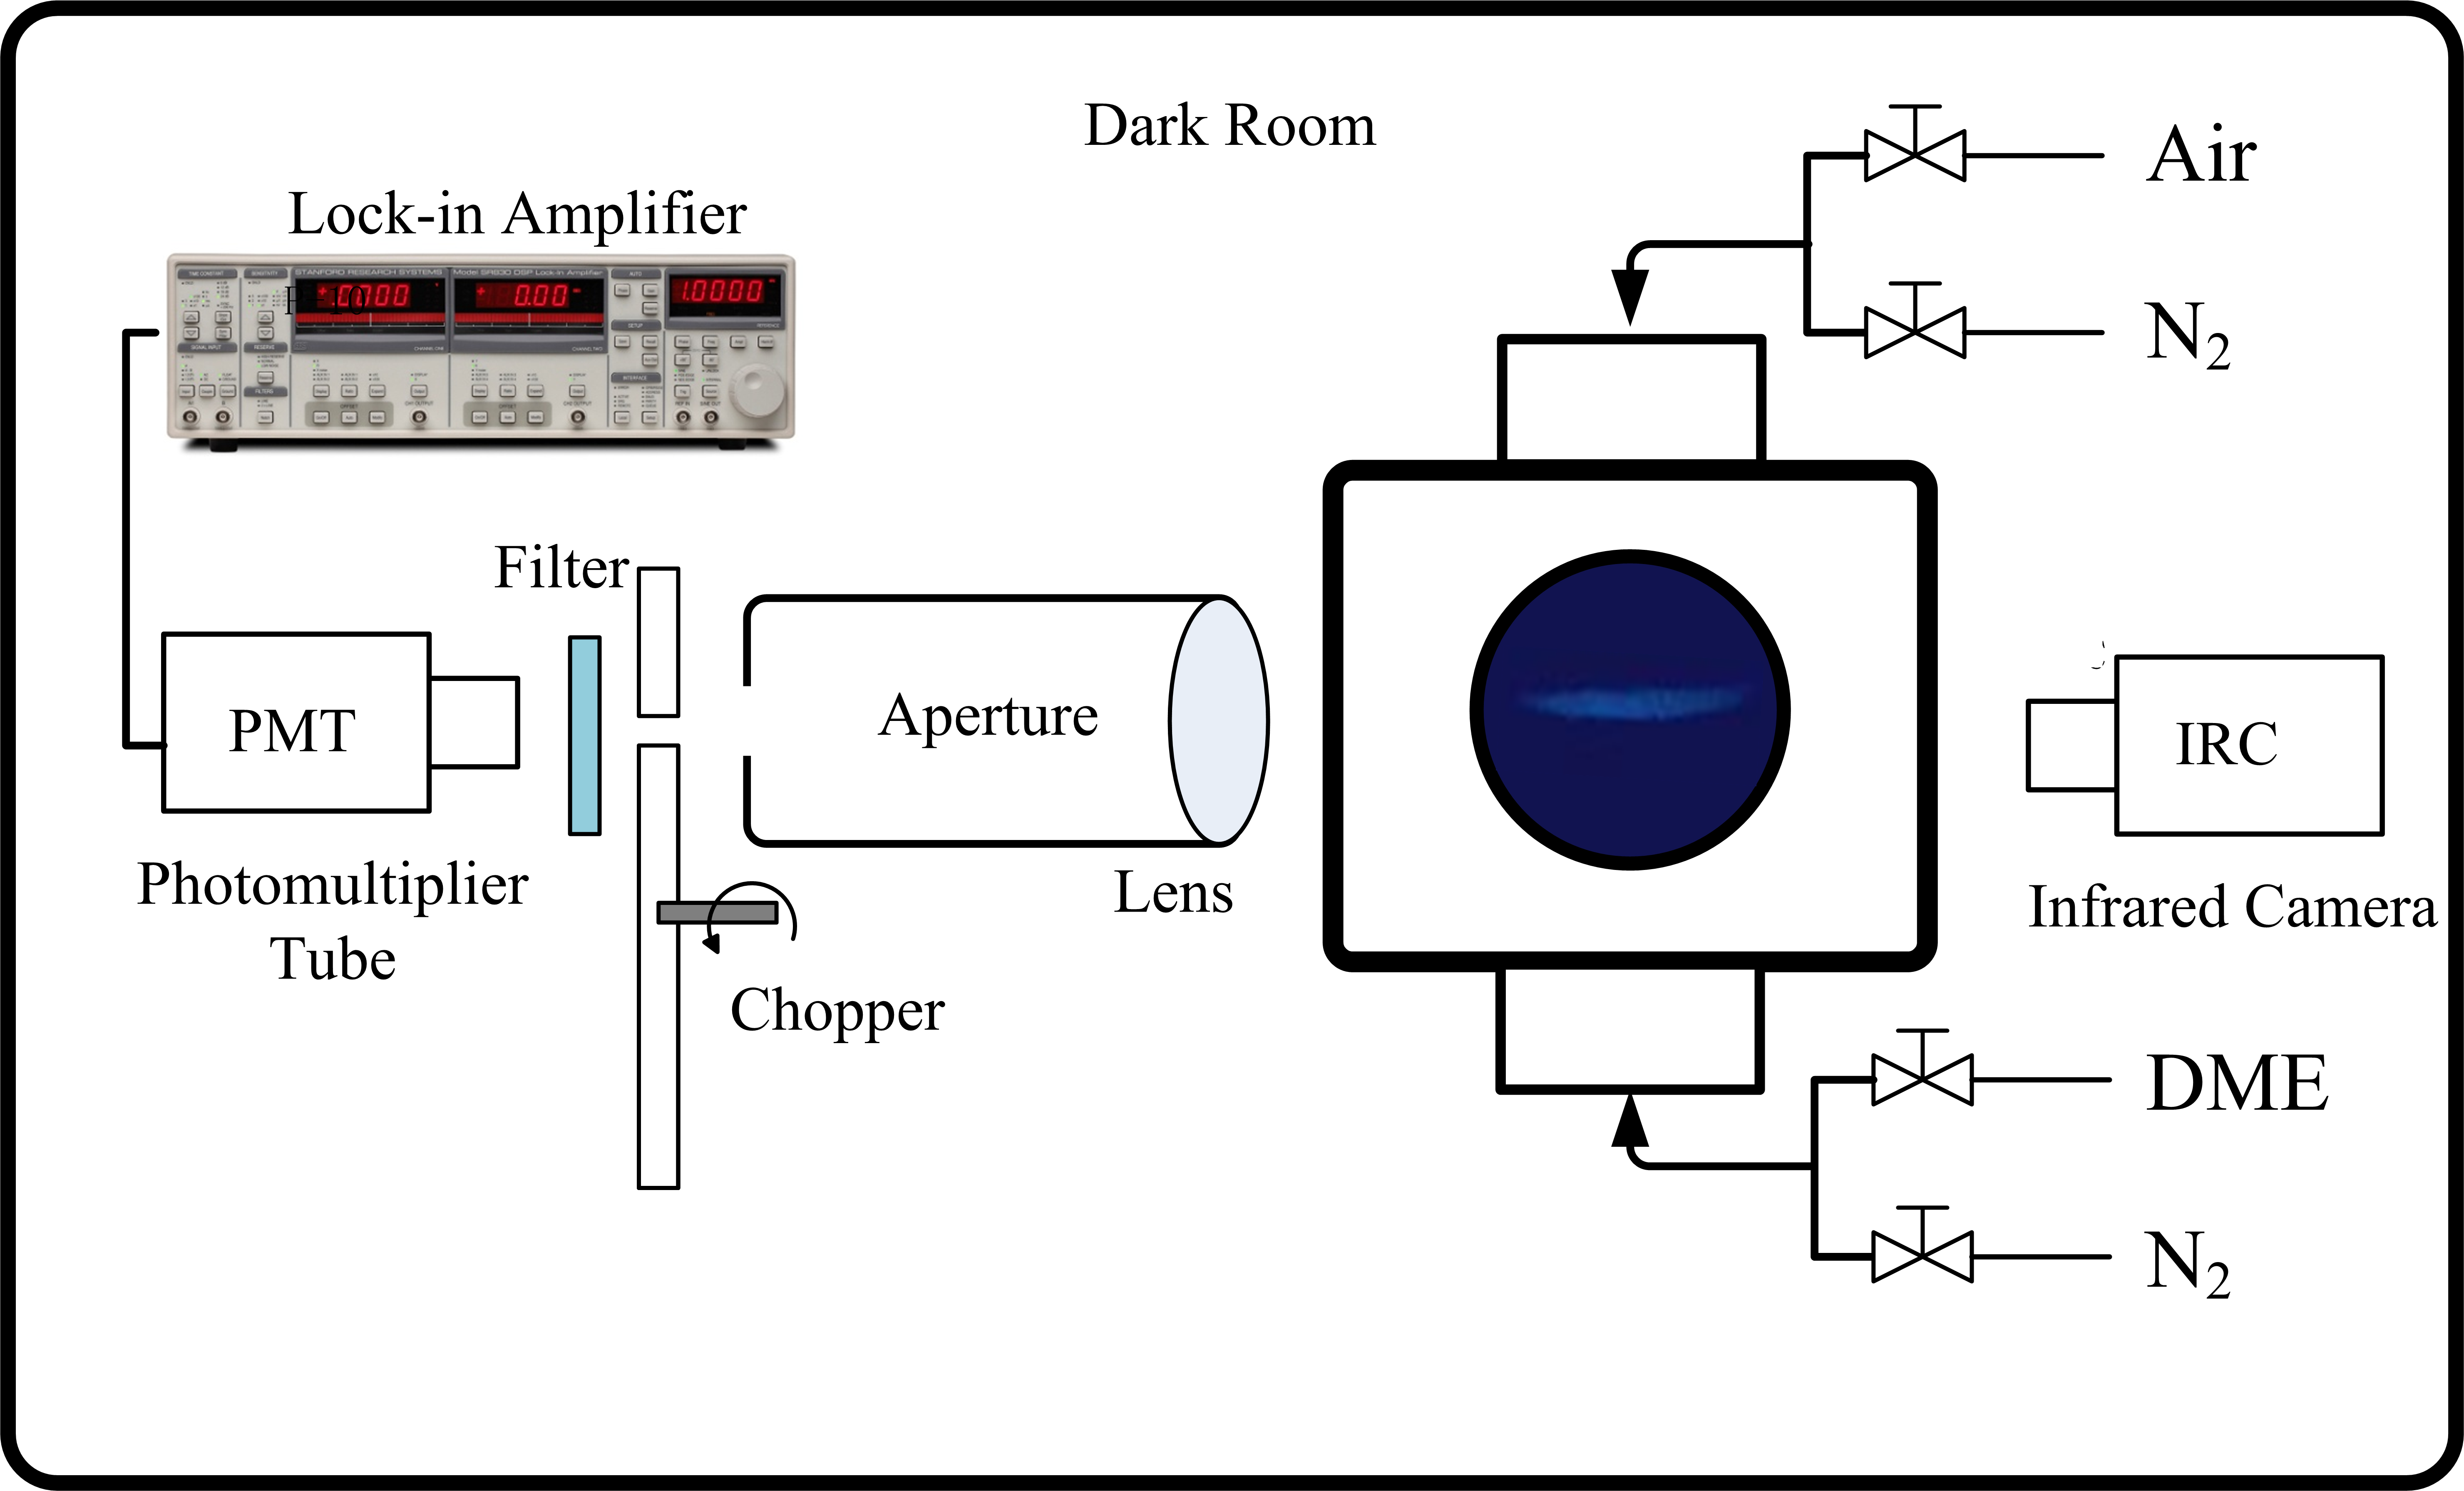
\includegraphics[width=0.8\textwidth]{Experimental_Setup.png}
  \normalsize
  \vspace{-0.1in}
  \caption{Schematic of the experimental system.}
  \label{fig:setup}
\end{figure}

While the above procedure has been successfully used in previous studies of ignition in the counterflow and stagnation flow, for which the instant of ignition can be observed visually, no bright flame or visually-detectable reaction front could be observed for the present NTC-affected ignition of DME within the temperature range of interests ($600-800$ K). 
As a first trial, a K-type thermocouple was used to measure the temperature profile and capture the heat release; however, no discernible heat release was captured, which might due to the small amount of heat release from the low temperature chemistry under the experimental condition and more possibly, the disturbance that the thermocouple introduced to the ignition kernel.  To avoid such disturbance, nonintrusive measurements by a photomultiplier tube (PMT)  were  then applied to detect the chemiluminescence at the state of ignition.  It is noted that experimental studies in homogeneous systems have shown that the NTC-induced cool flames have characteristic chemiluminescence spectra, as well as relatively small amount of heat release compared with hot flames~\cite{sheinson73,ohta91}.  These studies further show that a large amount of formaldehyde (HCHO) is formed from low temperature chemistry and the pale blue chemiluminescence from HCHO characterizes the cool flame~\cite{gaydonbook}.  Based on these characteristics, we designed our experiment as shown in Fig.~\ref{fig:setup}. Here a Hamamatsu 931B PMT combined with focusing lens and a Newport filter (10BPF10-400) was used to detect the chemiluminescence corresponding to the characteristic wavelength of formaldehyde (peaks around 400 nm) and reduce noise light signals from the counterflow chamber. The PMT signal was then collected and processed with a SR510 lock-in amplifier to further diminish the noise. 

Validation results for the experimental system are shown in Fig.~\ref{fig:M}.  When the PMT captures photons corresponding to the characteristic wavelength of HCHO (400 nm), it outputs negative impulses to the oscilloscope, with the amplitudes of these impulses represent the light intensity.  It is noted from Fig.~\ref{fig:M} that the such signal intensity drops after the replacement of either N$_2$-diluted DME with pure N$_2$ issued from the lower nozzle (at point a), or of air with N$_2$ issued from the upper nozzle (at point c), hence demonstrating that the signal is due to the presence of both air and DME. Since the replacement of air with the same flow rate of N$_2$ barely changes the temperature profile and the flow field, the signal difference between the air/DME and N$_2$/DME cases indicate the existence of NTC chemical activities.  It should be noted that, the weak signal from N$_2$/DME indicates chemiluminescence from thermal pyrolysis is minimal in this study, such that the difference in the chemical reactive and non-reactive cases should be mostly attributed to the low temperature oxidation chemistry.

To better visualize the flow field, an FLIR SC640 infrared camera was further used as shown on the right part of Fig.~\ref{fig:setup}, which was able to capture the infrared radiation from the ignition mixing layer.  The colors of the IR images indicate the IR radiation intensity, with the red color denoting higher radiation intensity than the blue color.  Unlike the chemiluminescence, both air/DME and N$_2$/DME cases radiate infrared signals when heated, due to the excitation of the vibrational modes of the gas molecules in the thermal mixing layer. However, above certain air boundary temperatures, discernible differences between the signal of the reactive air/DME case and that of the non-reactive N$_2$/DME case could be detected, which is caused by the thermal/radical runaway from the low tempearature chemistry.  Therefore, a criterion for the onset of the NTC-affected ignition can be set based on the IR camera observation. As the air boundary temperature gradually increases, the IR radiation intensity of N$_2$/DME flows is set as the reference state and compared with that of the air/DME signal. The C and D parts of Fig.~\ref{fig:IR} show the comparison of the air/DME chemically reactive and N$_2$/DME nonreactive cases at ignition. Ignition temperature measurement at the upper nozzle exit and LDV measurement for the local strain rate are then taken as mentioned above.


\begin{figure}[ht]
  \centering
  \scriptsize
  \vspace{-0.1in}
  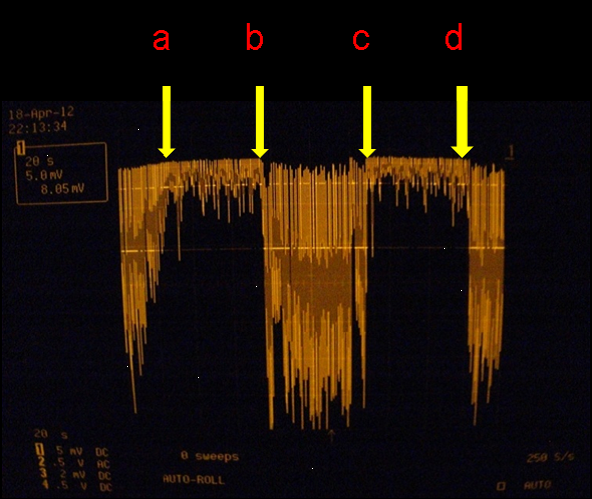
\includegraphics[width=0.5\textwidth]{M.png}
  \normalsize
  \vspace{-0.1in}
  \caption{"M" shaped signal. a.~Switch Air/DME to Air/N$_2$; b.~Switch Air/N$_2$ to Air/DME; c.~Switch Air/DME to N$_2$/DME; d.~Switch N$_2$/DME to Air/DME.}
  \label{fig:M}
\end{figure}

\begin{figure}[ht]
  \centering
  \scriptsize
  \vspace{-0.1in}
  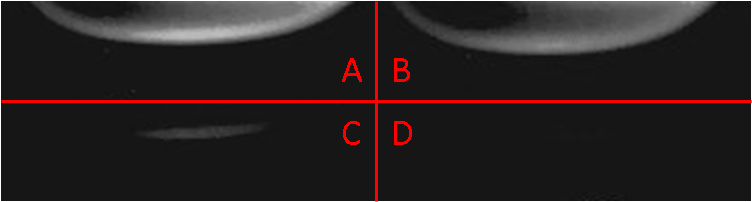
\includegraphics[width=0.5\textwidth]{IR.png}
  \normalsize
  \vspace{-0.1in}
  \caption{A/B: Heated air or N$_2$ against DME counterflow IR images; C/D: heated air or N$_2$ against DME counterflow IR images at ignition (atmospheric pressure, strain rate $60$ /s)}
  \label{fig:IR}
\end{figure}

\section{Computational Investigation}

The steady-state response of a one-dimensional reactive system subjected to heat loss can be studied via the S-curve analysis~\cite{lawbook}. In such an analysis, a system response such as the maximum temperature or radical concentration is monitored for variations of an imposed parameter such as the air temperature (for a given strain rate of the flow) or the system Damköhler number, which is defined as the characteristic flow time versus the characteristic chemical time. For a global one-step overall reaction with large activation energy, the intrinsically nonlinear Arrhenius kinetics frequently yields multiple solutions characterized by an S-shaped response curve when a system response is plotted against the system Damköhler number, with the lower and upper turning points respectively designate the ignition and extinction states of the system. Such triple-branch S-curves also frequently emerge for simulations using detailed reaction mechanisms, although more complex response curves with multiple ignition-extinction turning points have been obtained, for example for hydrogen oxidation~\cite{kreutz94,fotache98} and methane oxidation~\cite{liu09}. 

The governing equations for the counterflow nonpremixed flame are discussed in Giovangigli \emph{et al.}~\cite{giovangigli87}. The numerical code is modified from Smooke \emph{et al.}~\cite{smooke86}. It employs the damped Newton’s method and time integration solution scheme to solve the ordinary differential equations with boundary conditions specified on both sides of the potential flow. The S-curve marching is performed using the flame-controlling method of Nishioka \emph{et al.}~\cite{nishioka96} with detailed chemistry~\cite{kee89} and transport database~\cite{kee83}.

The critical states of ignition and extinction can then be assessed through the multiple turning points of the S-curve. The simulation conditions are as follows: the fuel-side mixture consists of DME and nitrogen with a fixed temperature of $300$ K, and the oxidizer side is standard air at a high temperature. The separation distance between the two nozzle exits is $20$ mm, with the origin being fixed at the fuel exit. To generate an S-curve, marching is performed by either changing the air-side boundary temperature with fixed strain rate or equivalently changing the strain rate with fixed air-side boundary temperature. Following Law and Zhao~\cite{law12,zhao13}, the distinct turning points of the NTC S-curve of DME were captured, and the calculated ignition temperature at different strain rates as well as different boundary fuel concentrations are compared with the  experimental results.

\section{Results and Discussion}

In Fig.~\ref{fig:Scurve-SR}, the global response of the system is chosen to be the maximum formaldehyde (HCHO) mole fraction due to its large production rate by the low temperature chemistry, and the NTC S-curve is plotted as a function of air boundary temperature for $30\%$ DME in nitrogen under different strain rates. It is noted that the second ignition state induced by the high temperature chemistry is not shown here. Then, it is seen that the ignition turning point for the NTC S-curve appears at the lower boundary temperature for lower strain rates, although the response is not as sensitive as the extinction turning point. In addition, the low temperature chemistry becomes more pronounced for lower strain rates as seen from the increasing maximum HCHO mole fraction for lower strain rates.

\begin{figure}[ht]
  \centering
  \scriptsize
  \vspace{-0.1in}
  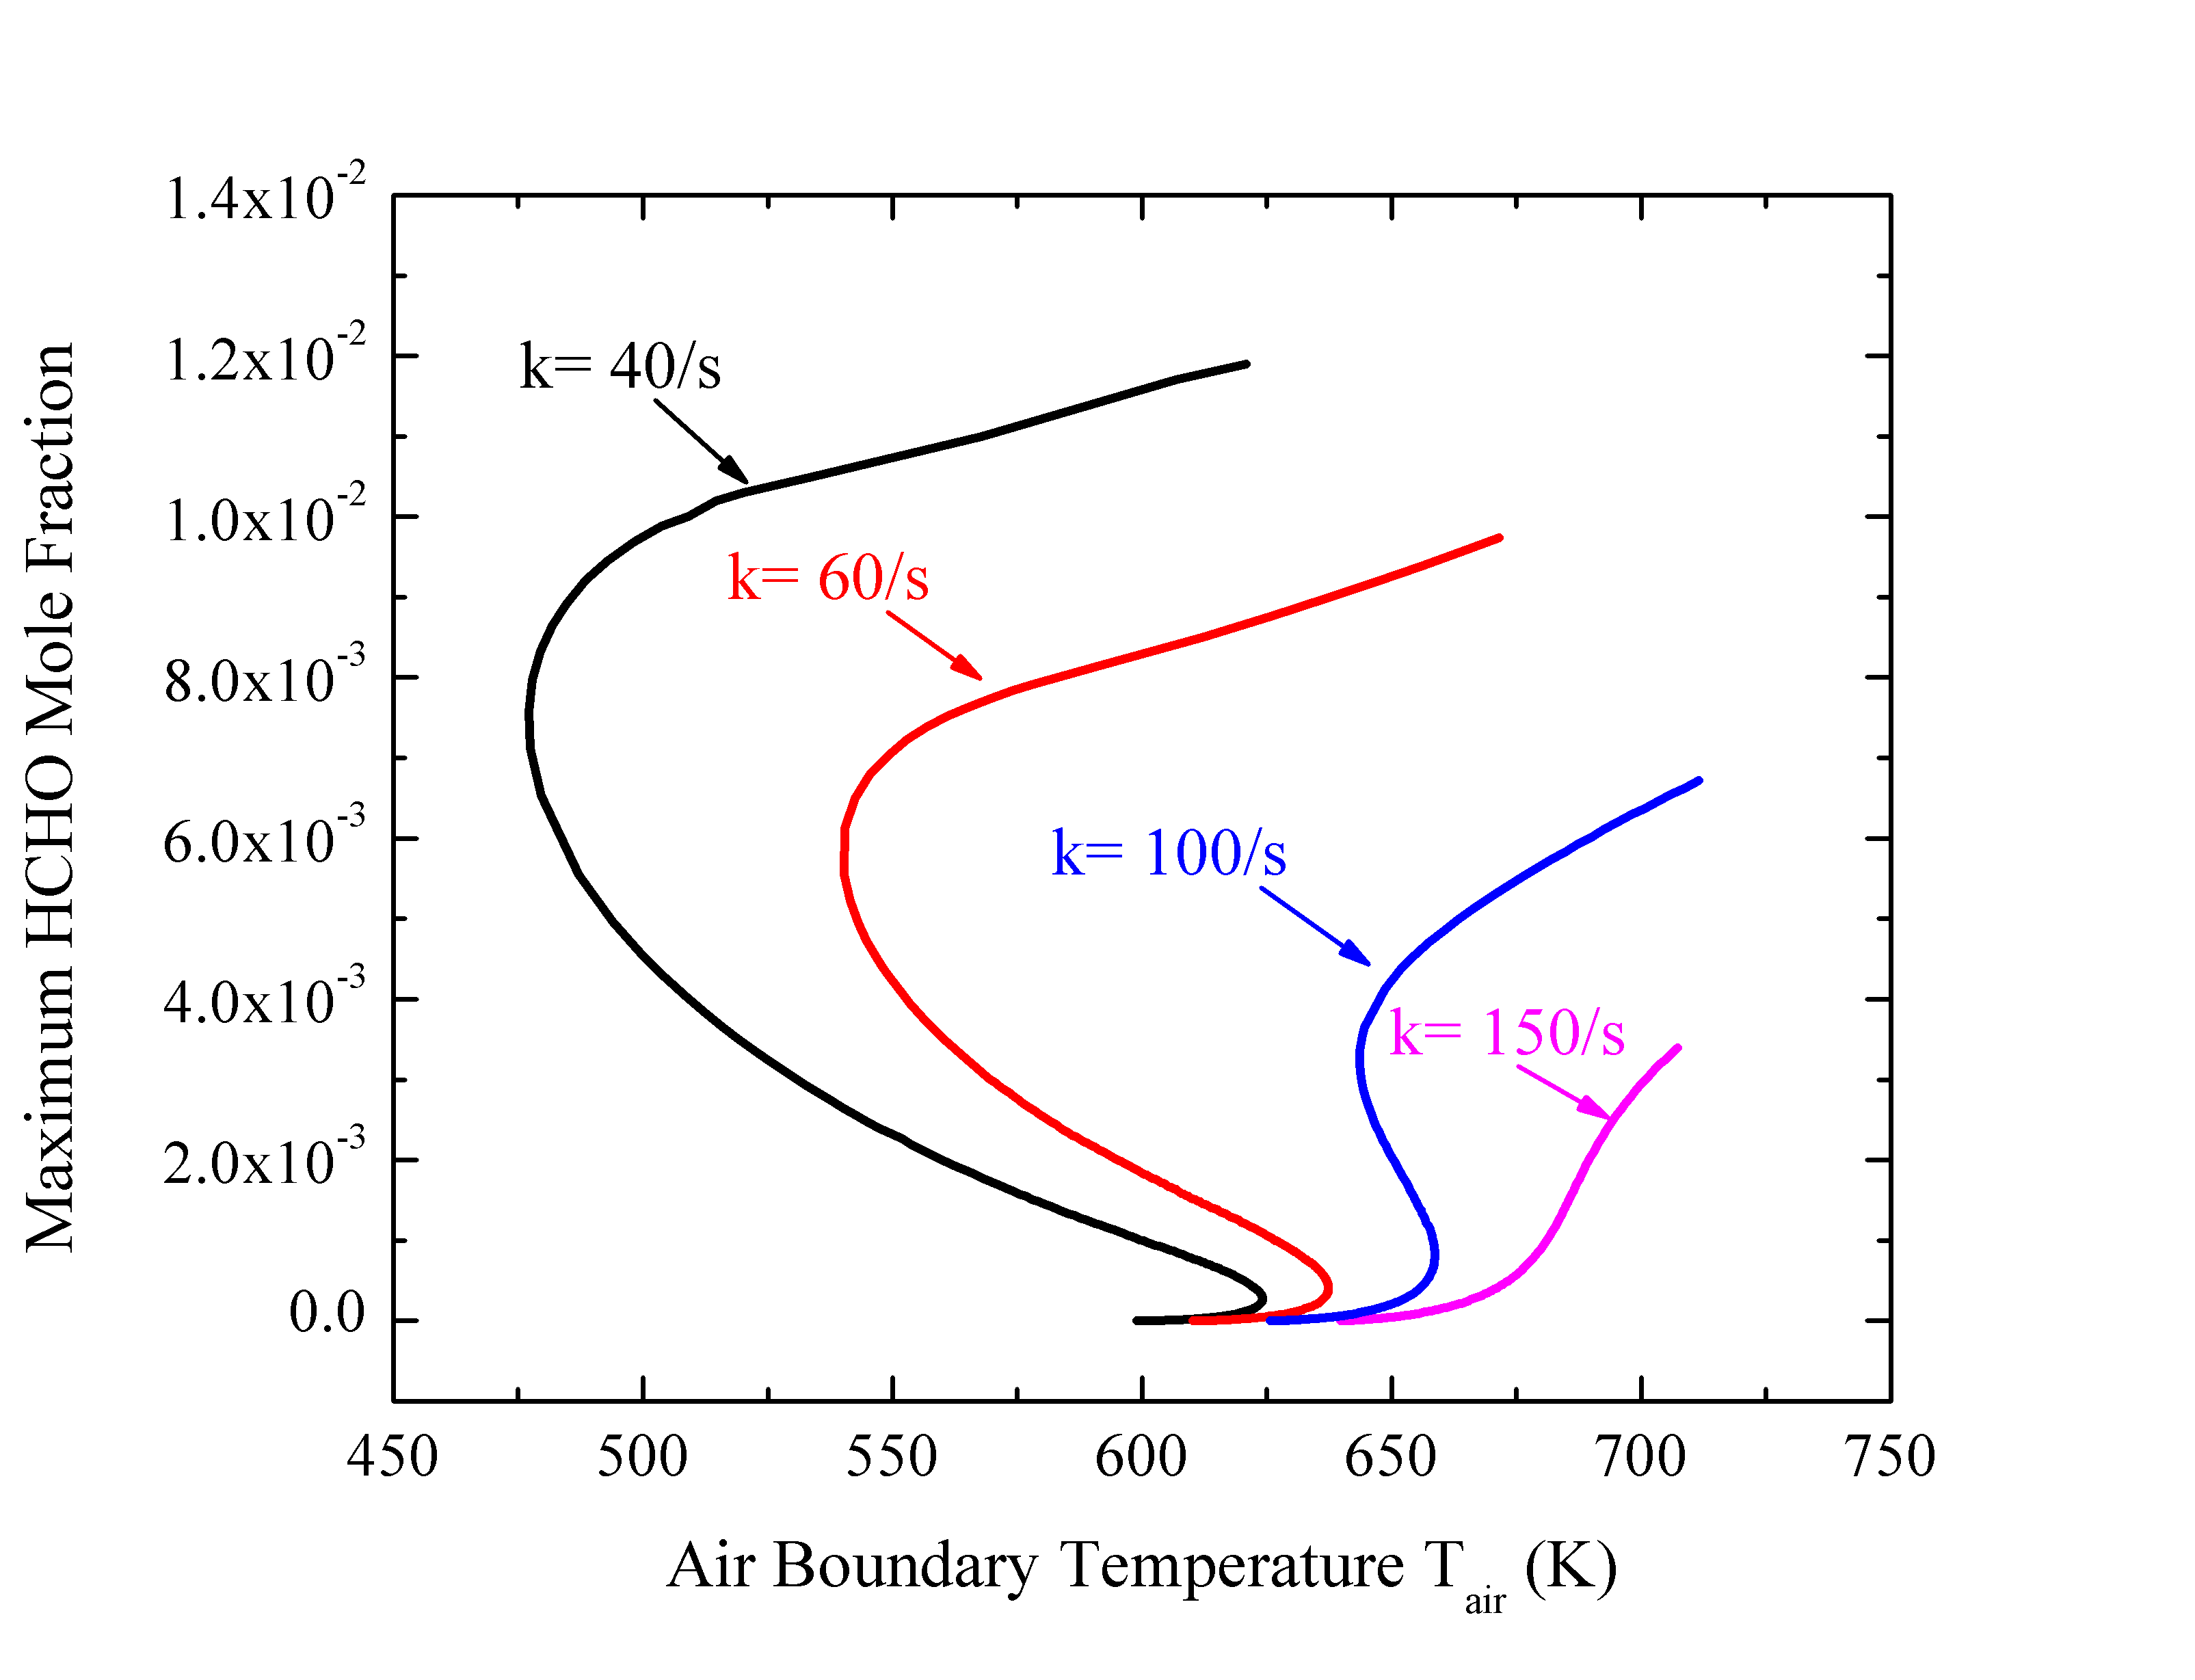
\includegraphics[width=0.6\textwidth]{Scurve-SR.png}
  \normalsize
  \vspace{-0.1in}
  \caption{Maximum HCHO mole fraction of $30\%$ DME at different air boundary temperatures under various strain rates.}
  \label{fig:Scurve-SR}
\end{figure}

For the experimental investigation, PMT with special filter for HCHO is used to measure the HCHO chemiluminescence intensity from the mixing layer. In Fig.~\ref{fig:PMT}, the chemiluminescence intensity from the HCHO under strain rates $40$ /s, $60$ /s, and $100$ /s are measured as a function of the air boundary temperature. Compared with Fig.~\ref{fig:Scurve-SR}, it again demonstrates that the low temperature chemistry becomes more pronounced under lower strain rates, with more HCHO produced and therefore stronger chemiluminescence from it. Consequently, though limited by system sensitivity, the signal can be detected at lower air boundary temperatures with decreasing strain rates. However, the current PMT system with HCHO filter fails to capture the onset of NTC-affected ignitions; instead, it shows the strength of chemiluminescence after ignition and at higher temperatures. It is also worth noticing that the discrepancy between the signal onset temperatures from experiment and NTC-affected ignition temperature from simulation is primarily due to the low intensity of HCHO chemiluminescence captured by the PMT. On the whole, qualitatively agreement of both stronger HCHO chemiluminescence as well as lower onset temperature detected with the numerical simulation does show the major characteristics of the NTC-transport coupling, which is consistent with previous work by Law and Zhao~\cite{law12}. 

\begin{figure}[ht]
  \centering
  \scriptsize
  \vspace{-0.1in}
  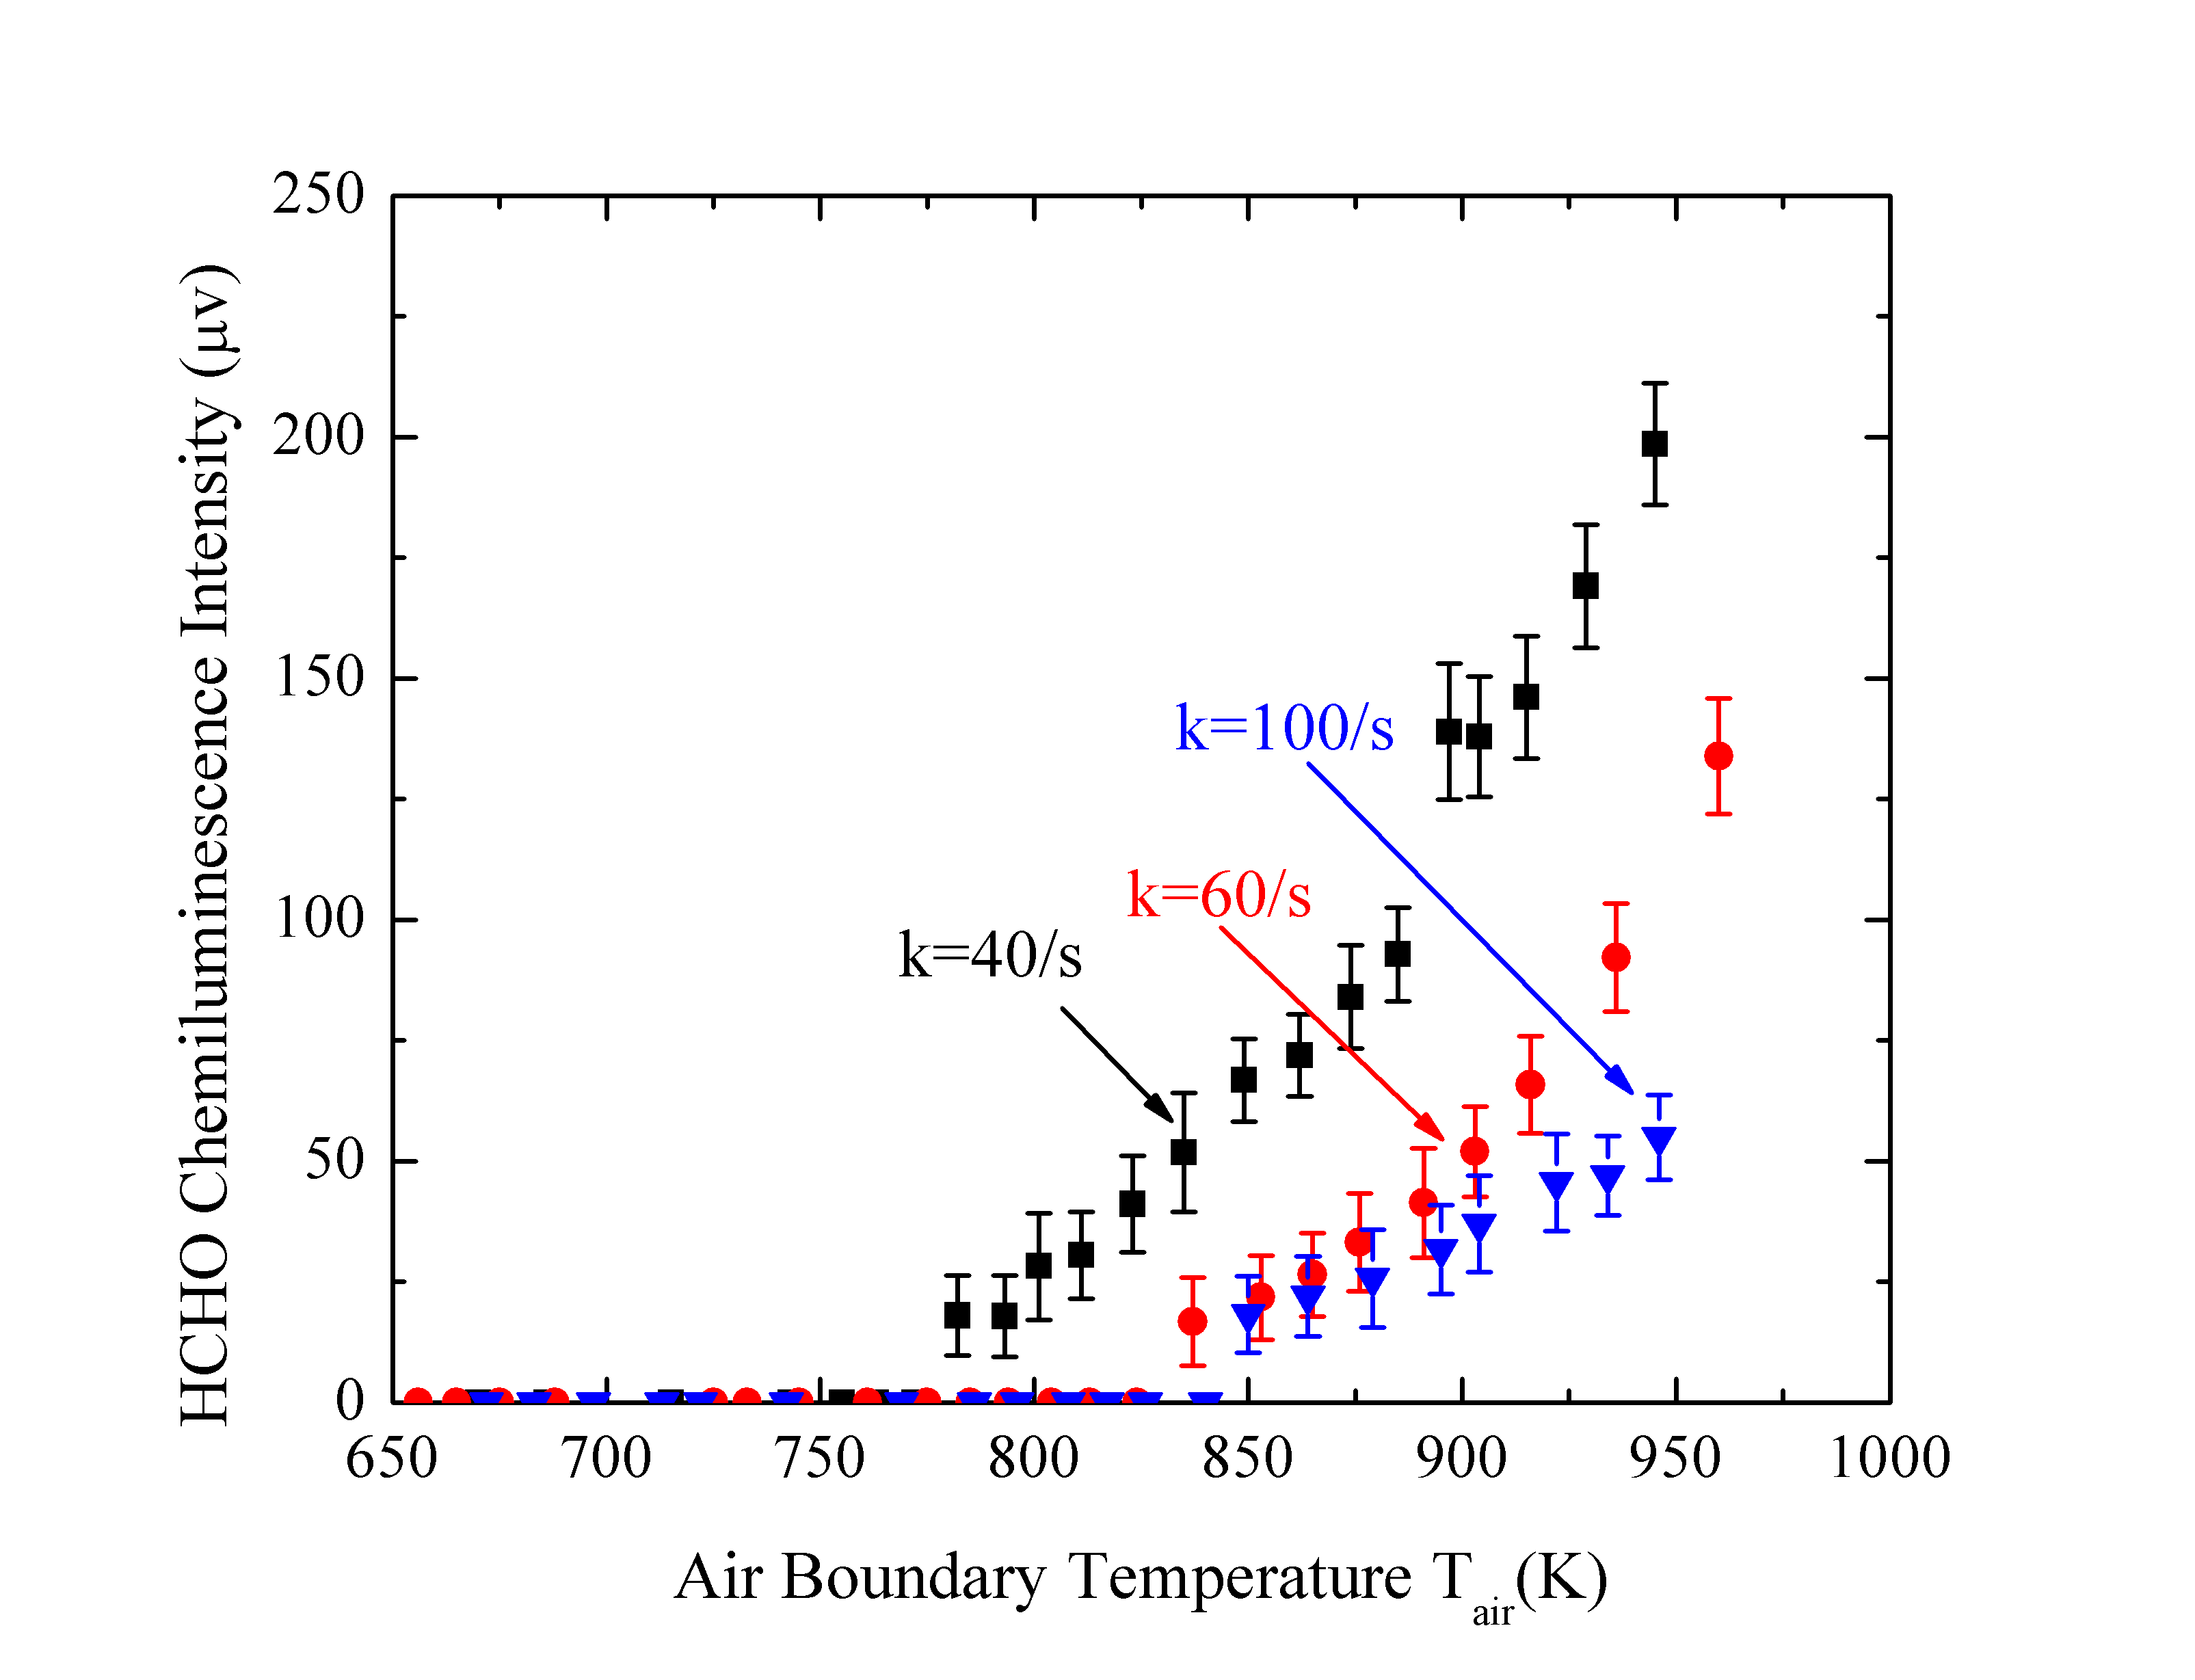
\includegraphics[width=0.6\textwidth]{PMT.png}
  \normalsize
  \vspace{-0.1in}
  \caption{HCHO chemiluminescence intensity at different air boundary temperatures under various strain rates.}
  \label{fig:PMT}
\end{figure}

As discussed in the experimental methodology section, quantitative measurement of the ignition temperature should be made based on the infrared camera observation. For different flow rates, the infrared camera was used to visualize the reaction mixing layer, and LDV was used to measure the velocity profile along the center line to further obtain the local strain rates of each case. In Fig.~\ref{fig:Ign-SR}, experimental measurements of the low temperature chemistry induced ignition and the turning points predicted by the NTC S-curve are plotted as function of strain rates. Due to the moderate flow field temperatures and high sensitivity of the thermocouple, ignition temperature error bars are within the size of the symbol. It is seen that very good agreement exists between the experimental observation and the numerical predictions, with the average temperature difference being within $20$ K. Sensitivity analysis was carried out to help understand the results and it is shown that the first two most important reactions for promotion of the low temperature chemistry induced ignition are oxygen combination reaction CH$_2$OCH$_2$O$_2$H+O$_2$ $\Leftrightarrow$ O$_2$CH$_2$OCH$_2$O$_2$H and isomerization reaction CH$_3$OCH$_2$O$_2$ $\Leftrightarrow$ CH$_2$OCH$_2$O$_2$H, and the most important retarding reaction is the $\beta$-scission reaction CH$_2$OCH$_2$O$_2$H $\Leftrightarrow$ OH+$2$HCHO. Clearly, these two groups of reactions compete for CH$_2$OCH$_2$O$_2$H radicals and function oppositely.

\begin{figure}[ht]
  \centering
  \scriptsize
  \vspace{-0.1in}
  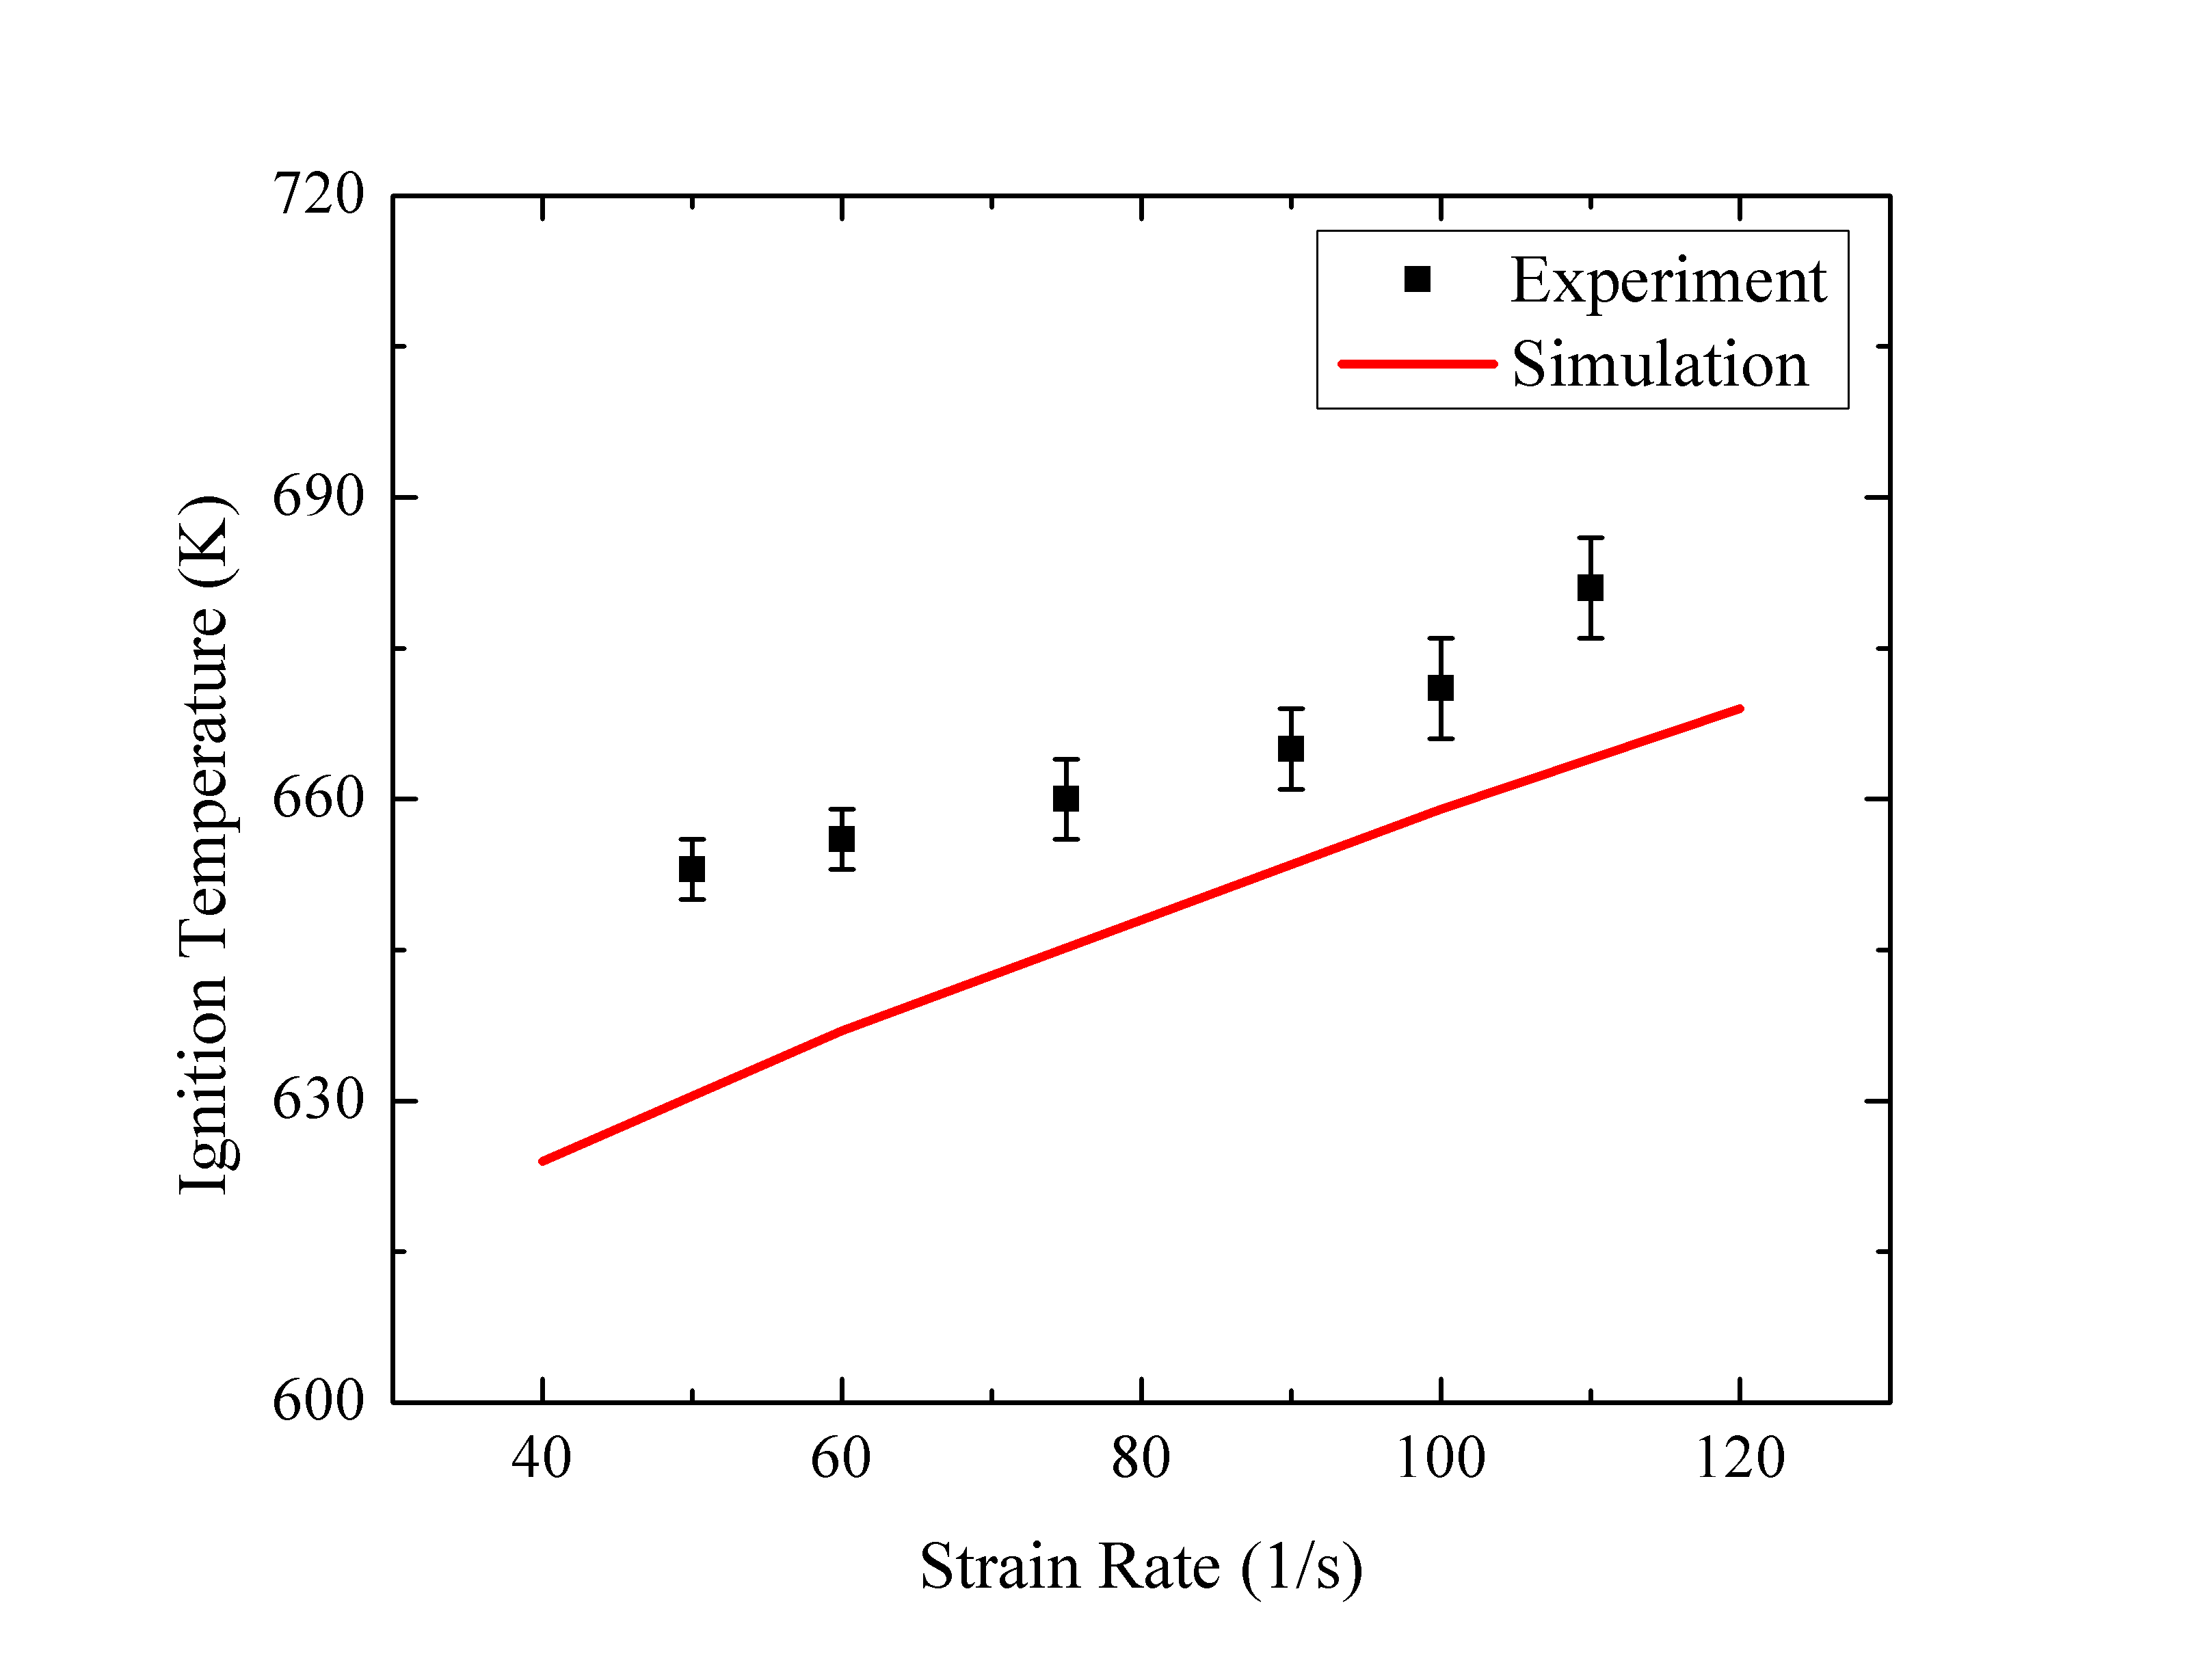
\includegraphics[width=0.6\textwidth]{Ign-SR.png}
  \normalsize
  \vspace{-0.1in}
  \caption{Calculated and observed ignition temperatures of $30\%$ DME under various strain rates.}
  \label{fig:Ign-SR}
\end{figure} 

In addition to strain rate effects, the concentration effect is also evaluated, shown and compared with the simulation results in Fig.~\ref{fig:Ign-Con}. The simulation result basically demonstrates the insensitive nature of the NTC-affected ignition temperature to the variance of boundary DME concentrations in a large range, under a fixed strain rate of $60$ /s. The experimental results again show good agreement with the simulation results. This effect corresponds to the equivalence ratio insensitive nature of the low temperature chemistry, given the fact that first stage delay is insensitive to equivalence ratio in homogeneous autoignition process~\cite{zhao13}.

\begin{figure}[ht]
  \centering
  \scriptsize
  \vspace{-0.1in}
  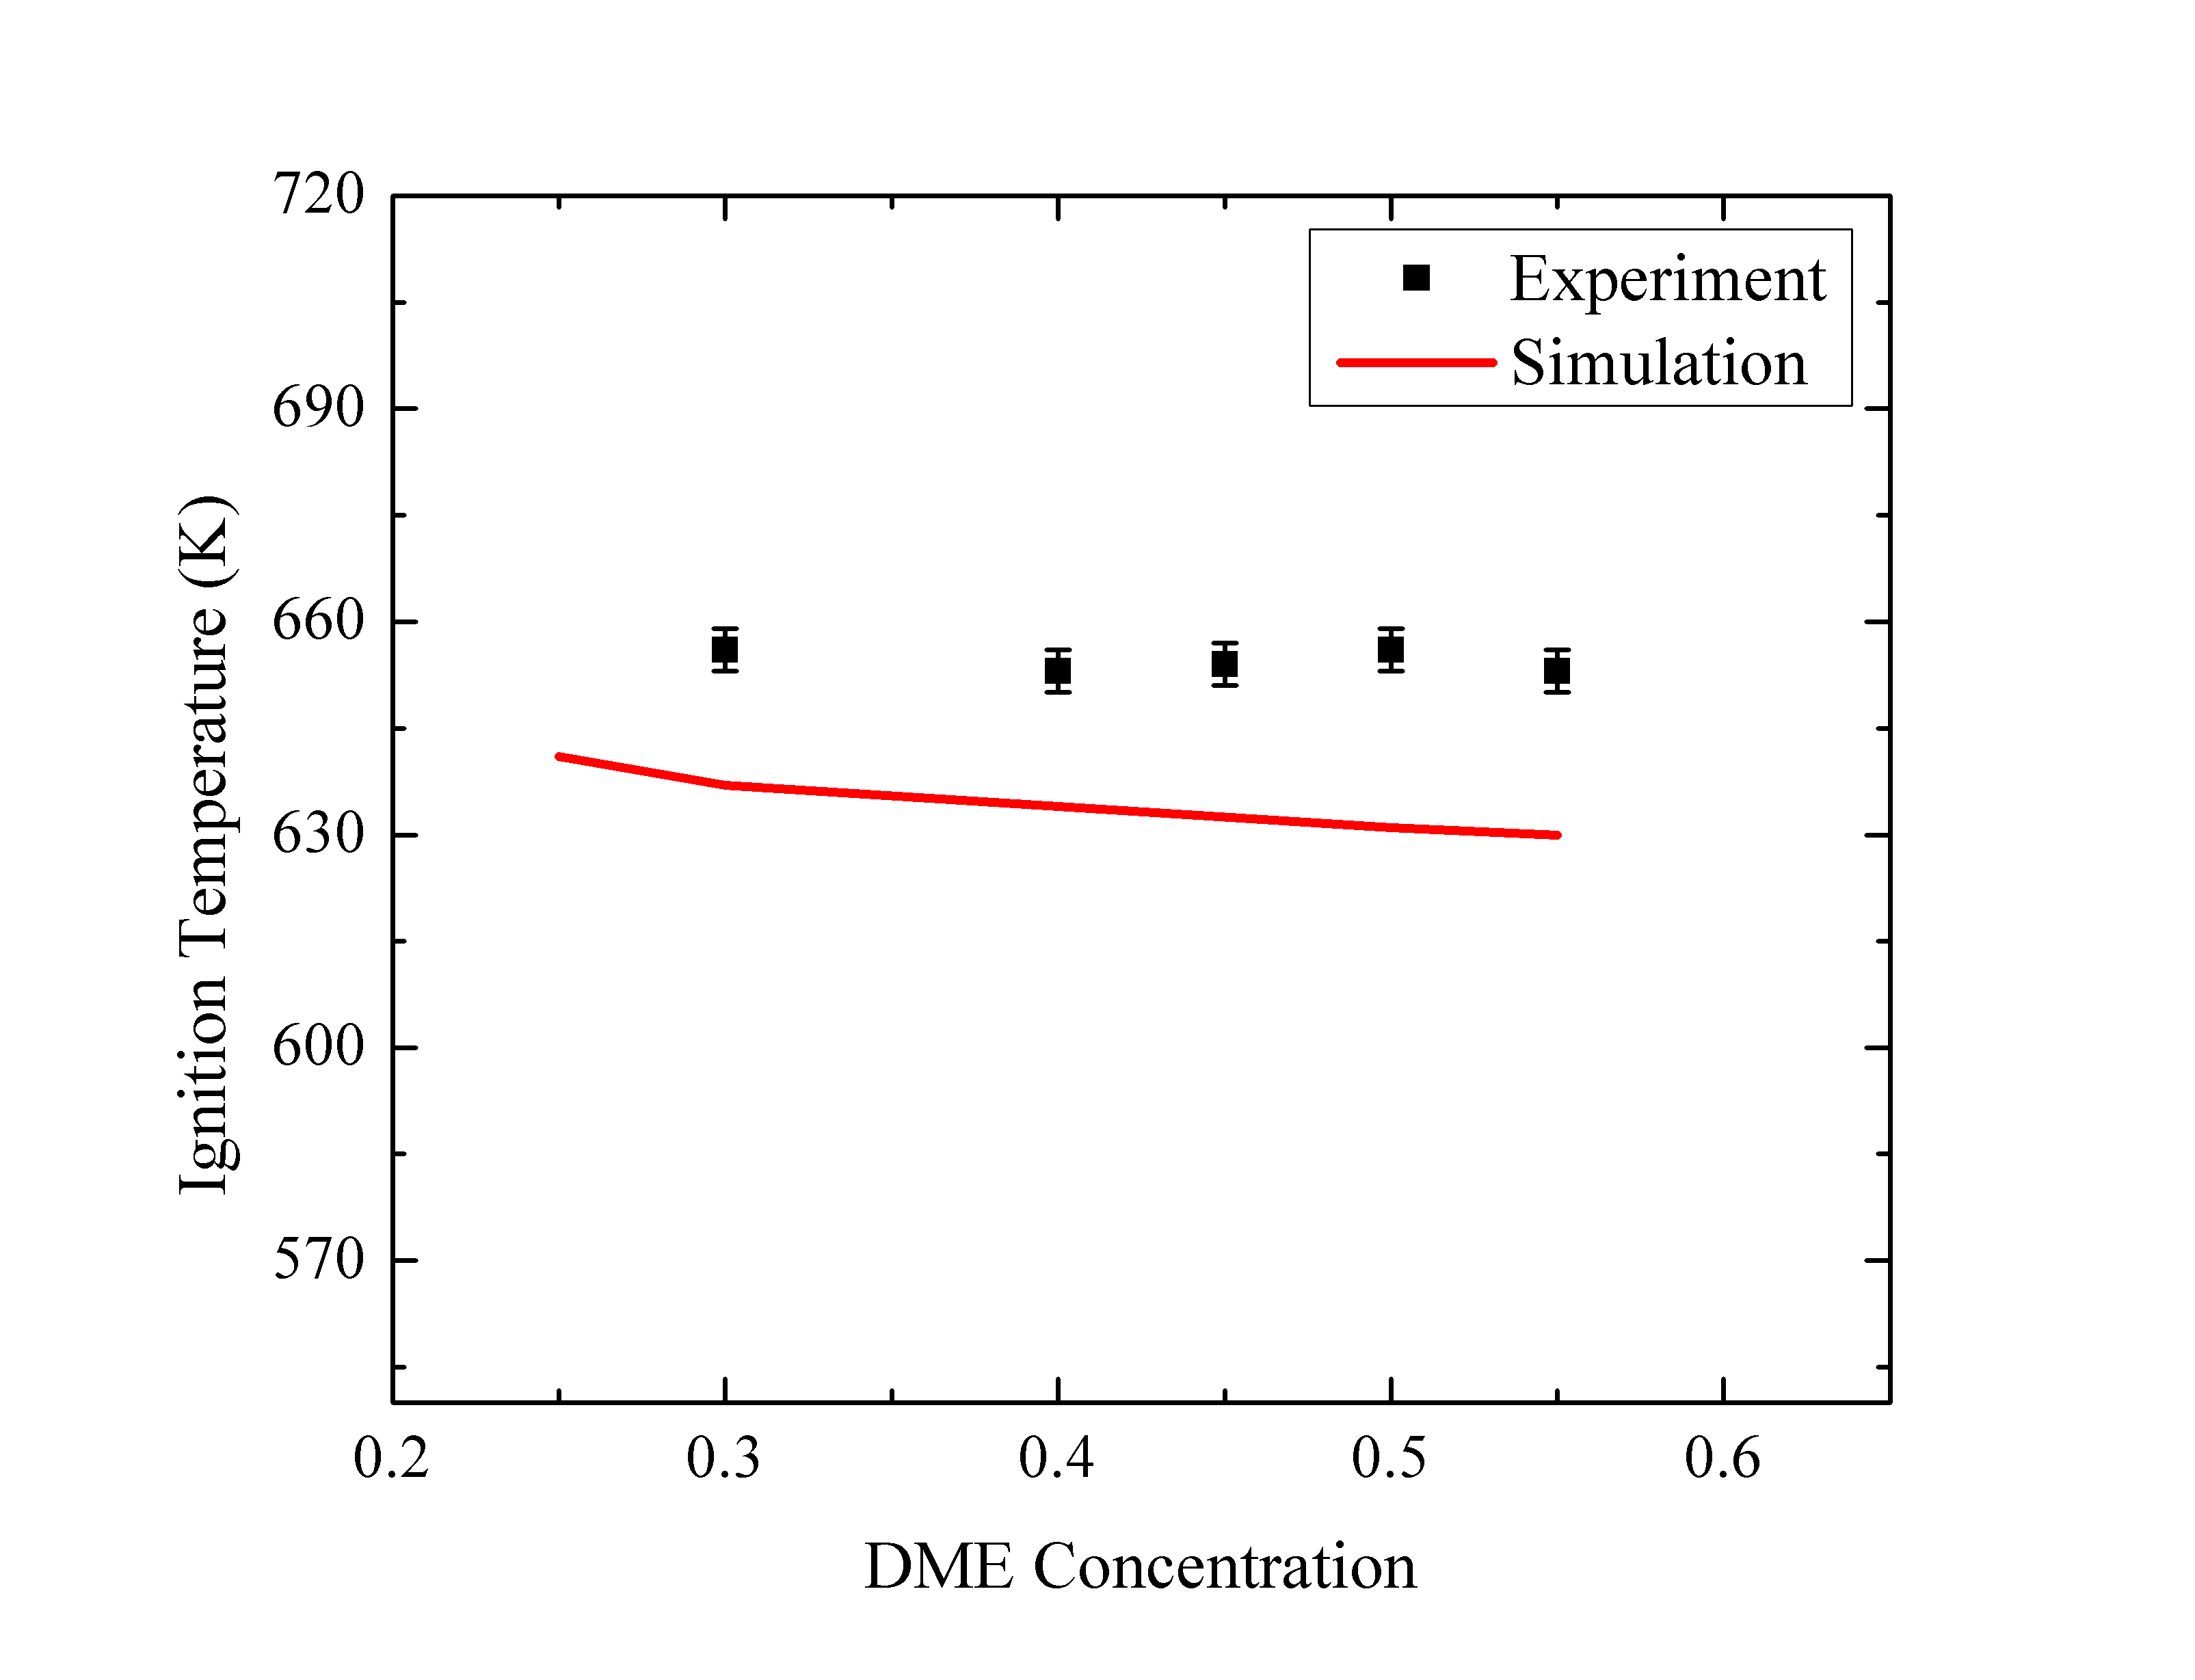
\includegraphics[width=0.6\textwidth]{Ign-Con.png}
  \normalsize
  \vspace{-0.1in}
  \caption{Ignition temperatures of various DME concentrations under the strain rate of $60$ /s.}
  \label{fig:Ign-Con}
\end{figure}

\begin{figure}[ht]
  \centering
  \scriptsize
  \vspace{-0.1in}
  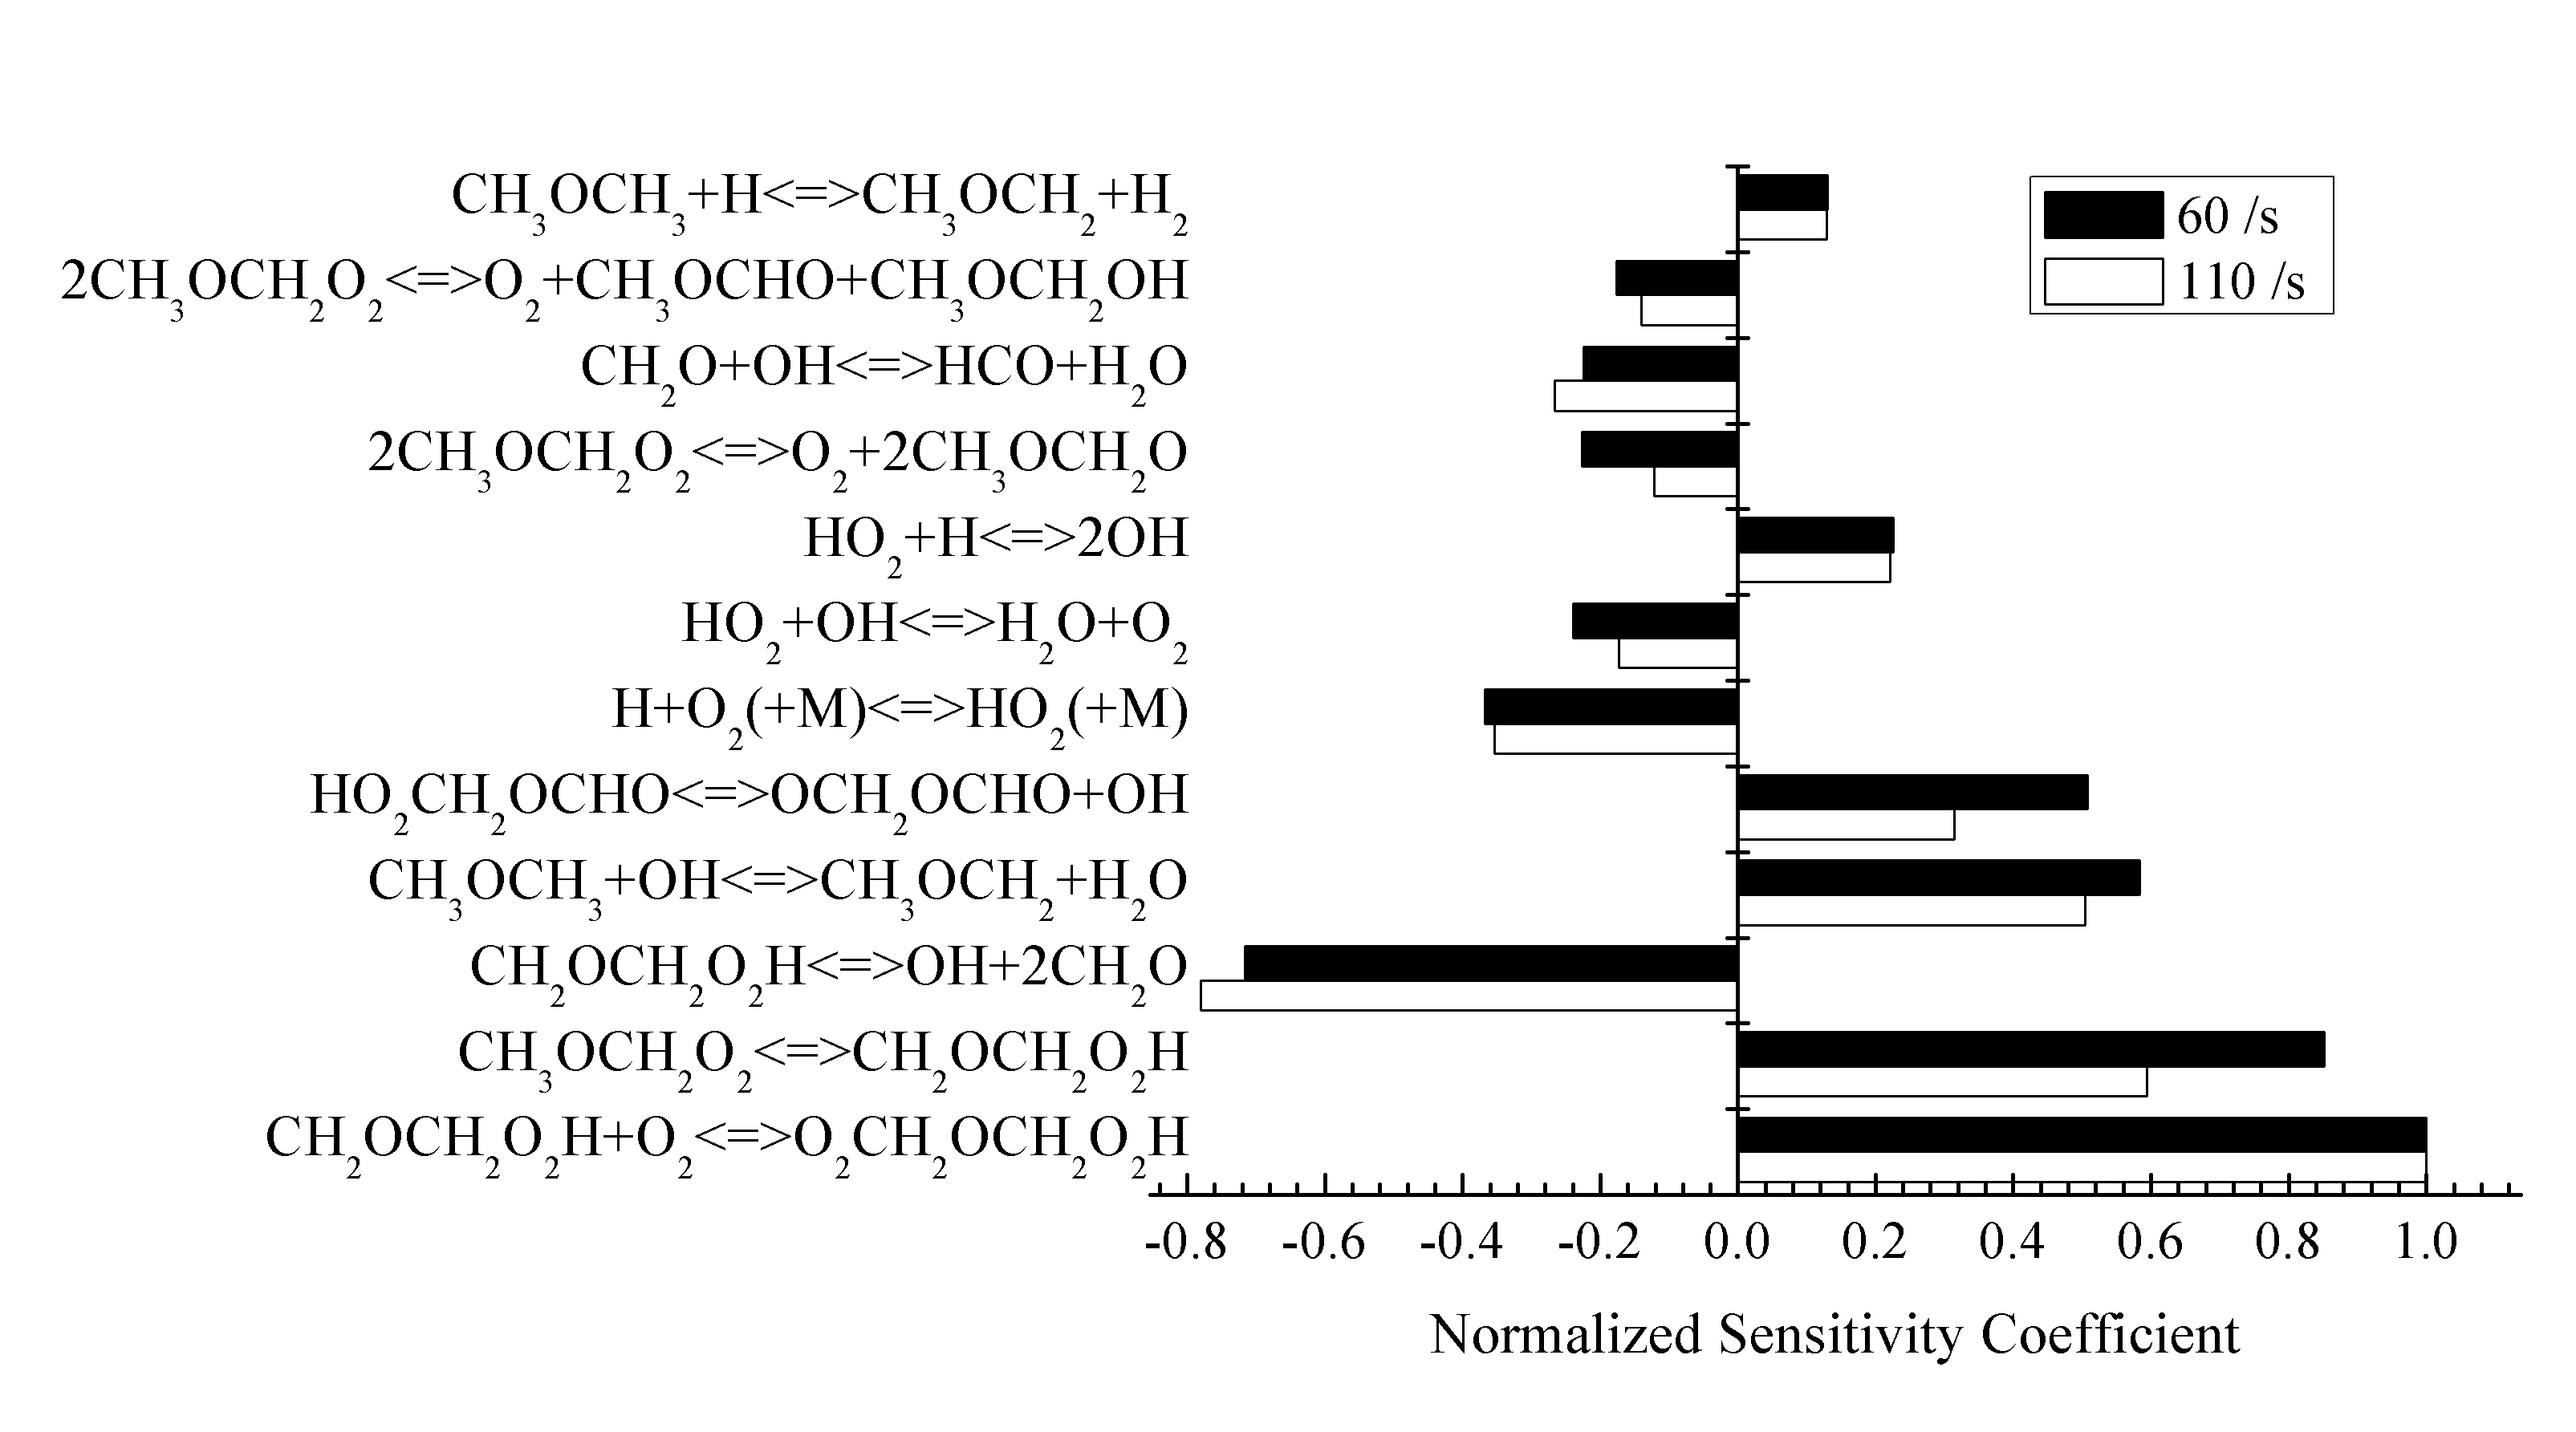
\includegraphics[width=0.7\textwidth]{Sen_SR.png}
  \normalsize
  \vspace{-0.1in}
  \caption{Sensitivity analysis on low and high strain rate cases: DME mole fraction is $30\%$.}
  \label{fig:Sen_SR}
\end{figure}


\begin{figure}[ht]
  \centering
  \scriptsize
  \vspace{-0.1in}
  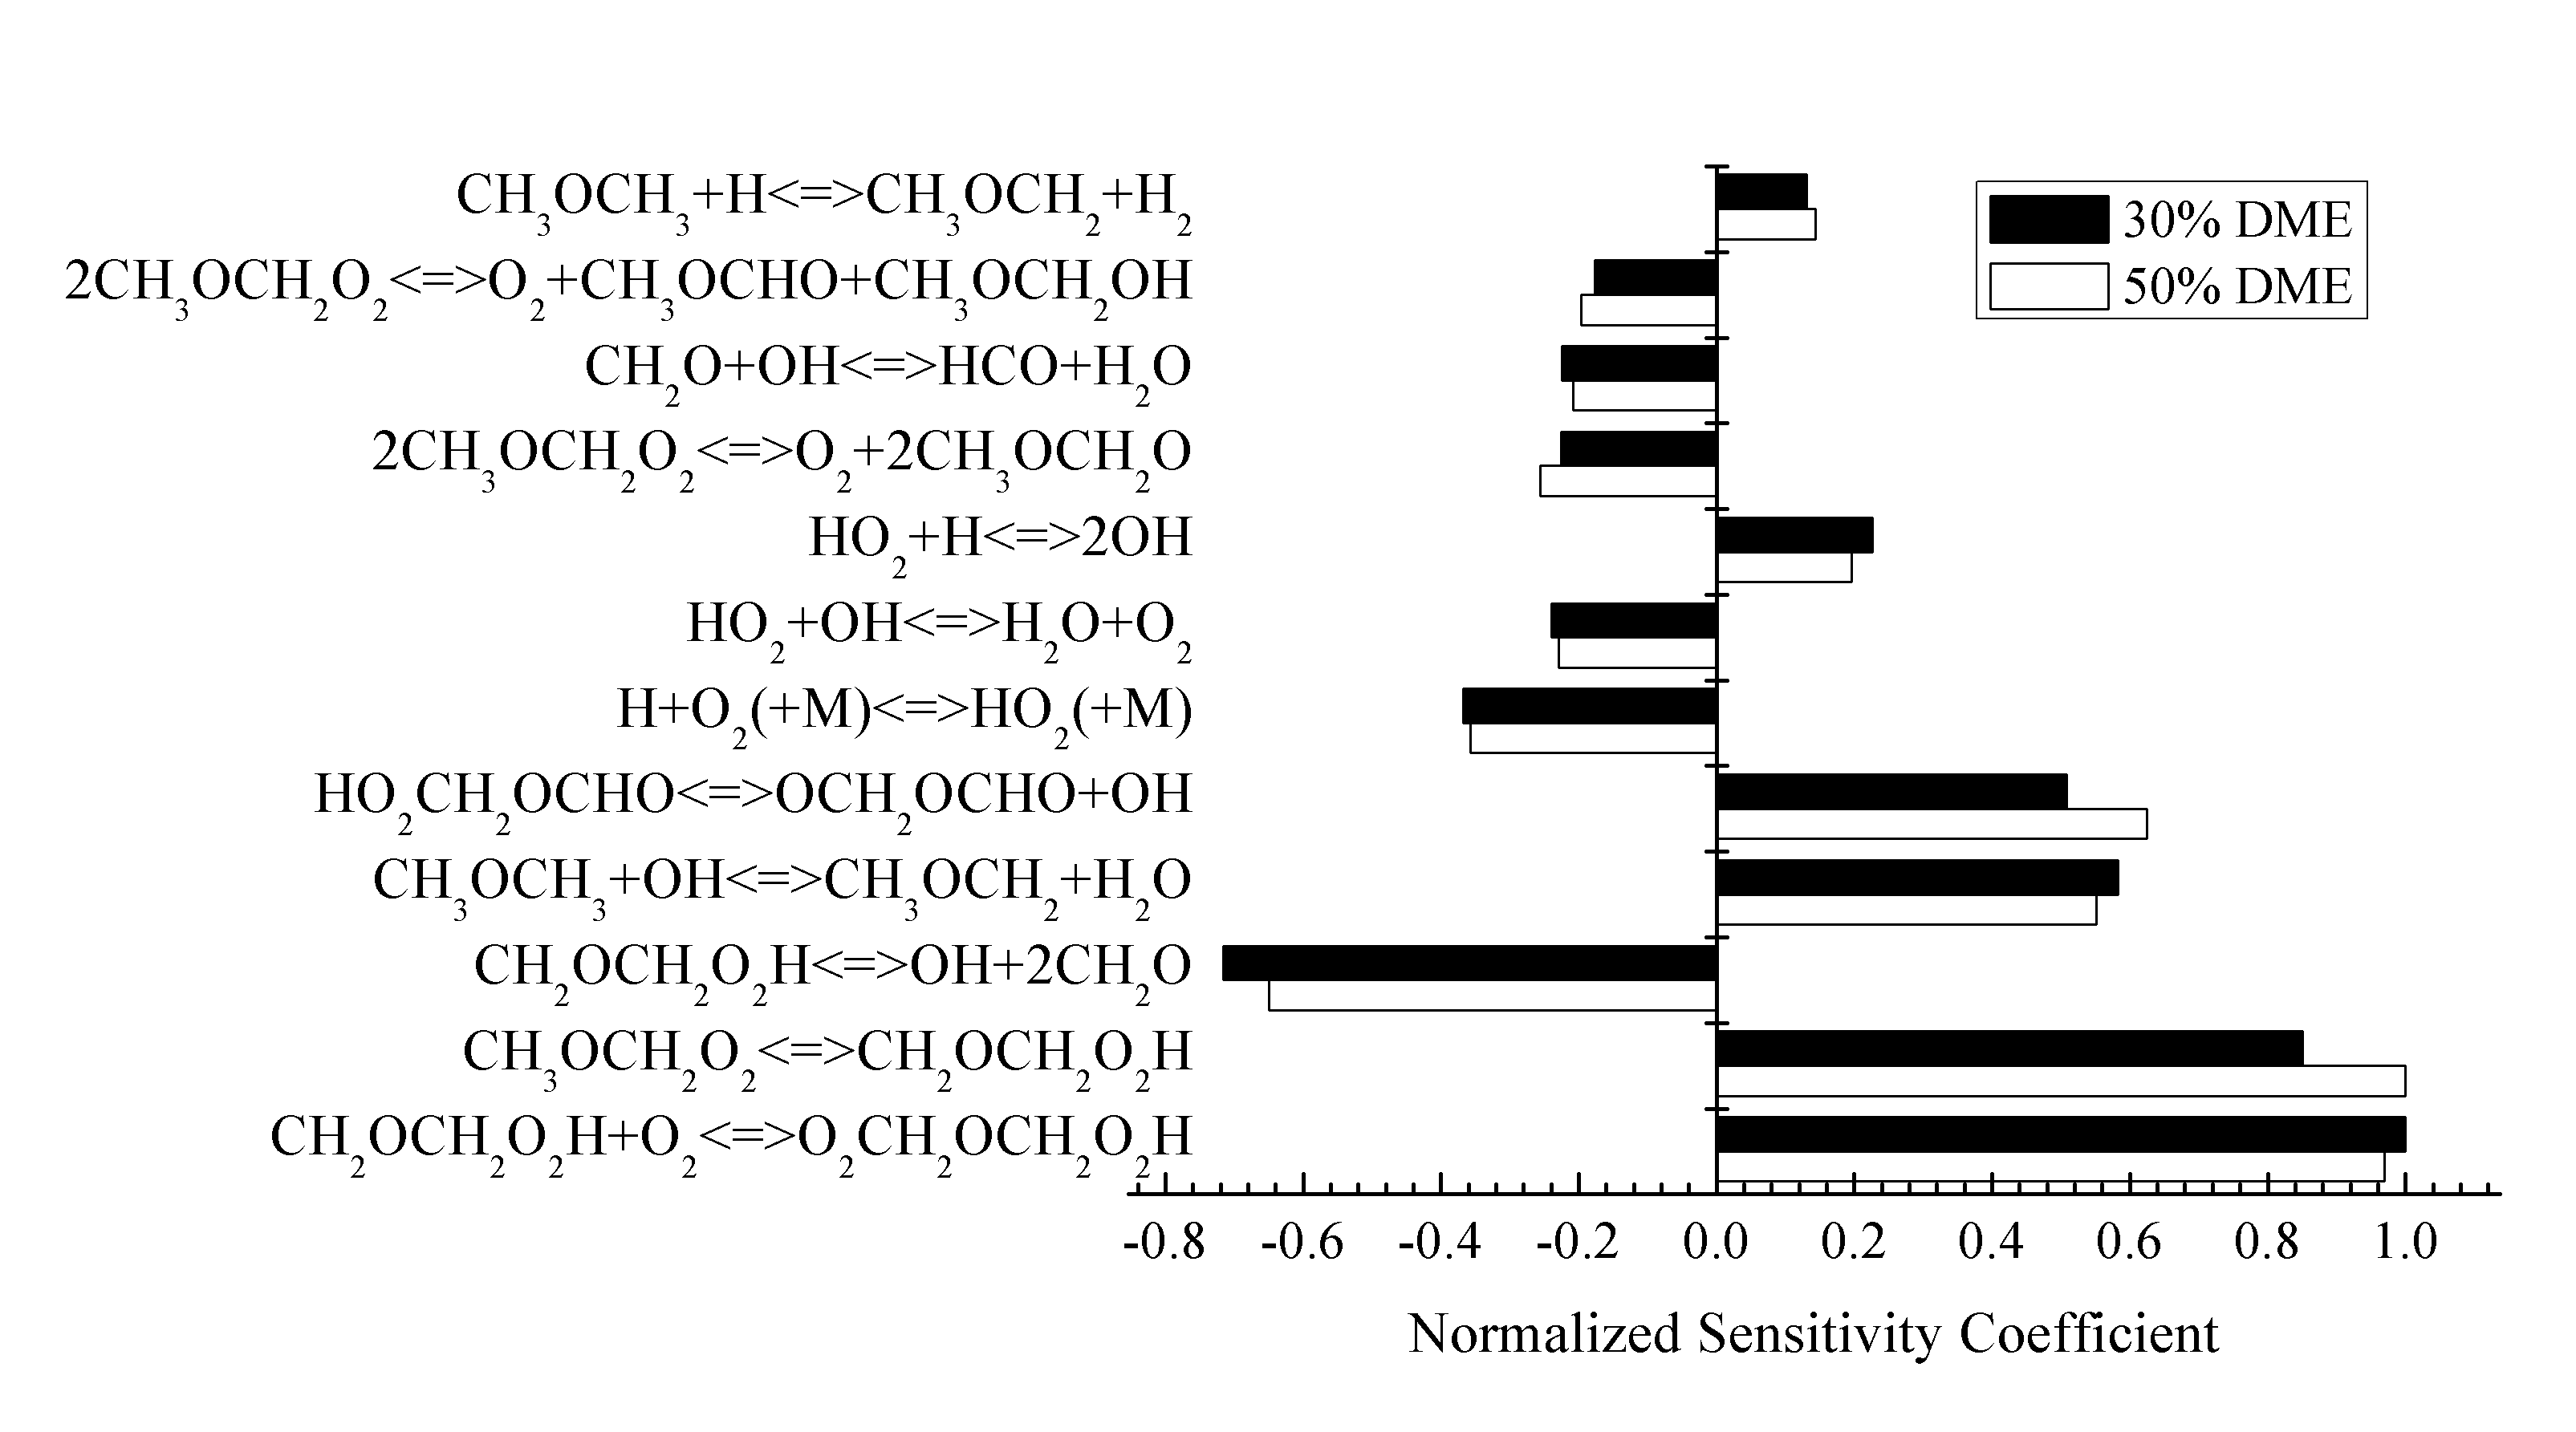
\includegraphics[width=0.7\textwidth]{Sen_Con.png}
  \normalsize
  \vspace{-0.1in}
  \caption{Sensitivity analysis on low and high DME concentration cases: the strain rate is  $60$ /s.}
  \label{fig:Sen_Con}
\end{figure}



\section{Conclusions}           

A photomultiplier tube and infrared camera were employed in the traditional nonpremixed counterflow system to investigate the NTC-chemistry and transport coupling in low temperature chemistry induced ignition, thus to demonstrate the existence of diffusion cool flame. The ignition temperatures, as well as chemiluminescence intensities from formaldehyde of different concentrations of DME in nitrogen under various strain rates were obtained. Both qualitative and quantitative agreements were achieved between the experimental investigation and the numerical simulation. 

It was found that with decreasing strain rates, the onset temperature for detectable chemiluminescence decreases, while the intensity for the chemiluminescence from the HCHO generated by the low temperature chemistry also becomes more pronounced. In addition, the ignition temperature of NTC-induced ignition was shown to increase with increasing strain rate and was insensitive to a wide range of boundary fuel concentrations. Such findings demonstrated the important features about low temperature chemistry and provided new tools to study low temperature chemistry and transport coupling process. 

\section*{Acknowledgments}
This work was supported by the Combustion Energy Frontier Research Center, an Energy Frontier Research Center funded by the US Department of Energy, Office of Basic Energy Sciences under Award Number DE-SC0001198.

\section*{References}
\bibliographystyle{elsarticle-num-CNF}
\bibliography{NTC}

\renewcommand{\thefigure}{\arabic{figure}}
\renewcommand{\thetable}{\arabic{table}}

\end{document}

